\maketitle

\cleardoublepage
\phantomsection
\addcontentsline{toc}{chapter}{Indice}
\tableofcontents

\listoffigures
\listoftables% TODO: \usepackage{graphicx} required
\lstlistoflistings

\chapter{Introduzione}
	\textsl{\textbf{Climate Monitoring}} \`e un'applicazione sviluppata nell’ambito del progetto di Laboratorio InterdisciplinareB (A.A. 2023/24) per il corso di laurea in Informatica dell’\textsl{Universit\`a degli Studi dell’Insubria} di Varese.
	
	Il progetto \`e sviluppato in \textsl{Java 17} sui sistemi operativi \textsl{Arch Linux} e \textsl{Windows 11}.
	L'applicazione \`e stata testata sugli stessi sistemi.
	\section{Librerie esterne utilizzate}
		Per lo sviluppo di questo progetto sono state utilizzate alcune librerie di terze parti.
	\subsection{\textsl{LIB1}}
\chapter{Database (dbCM)}
	Di seguito si mostra lo schema Entità-Relazione del database di supporto all’esecuzione dei servizi della piattaforma Climate Monitoring.
	
	\begin{figure}[h]
		\centering
		\caption{Schema ER di dbCM}
		\label{fig:erdb}
		\includegraphics[width=0.8\linewidth]{../../../myfiles/database/ERdb}
	\end{figure}
	
	In questo schema vegono illustrate le 4 entità richieste dalle specifiche e le relative associazioni.
	
	Nel dettaglio, le entità sono:
	\begin{itemize}
		\item \textbf{\textit{CentriRegistrati}}, contenente tutte le informazioni relative ai centri di monitoraggio registrati nel sistema, creati dai vari operatori;
		\item \textbf{\textit{CoordinateMonitoraggio}}, contenente i dati riguardanti le aree geografiche presenti nel documento "CoordinateMonitoraggio.xlsx" fornito nelle specifiche di progetto;
		\item \textbf{\textit{OperatoriRegistrati}}, racchiude i dettagli relativi gli operatori che hanno effettuato la registrazione al sistema;
		\item \textbf{\textit{ParametriClimatici}}, modella dei record per contenere tutte le informazioni che interessano le misurazioni effettuate in determinate aree d'interesse dagli operatori registrati, per conto dei relativi centri di monitoraggio.
	\end{itemize}
	\pagebreak
	Le associazioni costruite sulle entità appena elencate sono le seguenti:
	\begin{itemize}
		\item \textbf{\textit{"provides"}}, tra \textit{OperatoriRegistati} e \textit{ParametriClimatici}, con cardinalità \textbf{\textit{(0,n)-(1,1)}}
		
		Ogni operatore registrato può difatti fornire più misurazioni climatiche, mentre una misurazione può essere stata fornita da uno e un solo operatore registrato.
		\item \textbf{\textit{"related\_to"}}, tra \textit{ParametriClimatici} e \textit{CoordinateMonitoraggio}, con cardinalità \textbf{\textit{(1,1)-(0,n)}}
	
		Ogni misurazione climatica deve difatti essere relativa a una e una sola area geografica, mentre un'area geografica può avere associate molteplici misurazioni, come non averne.
		\item \textbf{\textit{"submits"}}, tra \textit{CentriMonitoraggio} e \textit{ParametriClimatici}, con cardinalità \textbf{\textit{(0,n)-(1,1)}}
		
		Ogni centro di monitoraggio può presentare più misurazioni relative alle proprie aree d'interesse, mentre una misrurazione deve essere stata resa disponibile da uno e un solo centro di monitoraggio.
		
		\item \textbf{\textit{"works\_in"}}, tra \textit{OperatoriRegistrati} e \textit{CentriMonitoraggio}, con cardinalità \textbf{\textit{(1,1)-(1,n)}}
	
		Ogni operatore deve associarsi a un centro di monitoraggio in seguito alla registrazione, se quello a cui vuole associarsi non è presente nel sistema, ne crea uno nuovo. In ogni centro di monitoraggio lavora almeno un operatore (il suo creatore), ed eventualmente altri associati.
		
		\item \textbf{\textit{"Area\_Center"}}, tra \textit{CoordinateMonitoraggio} e \textit{CentriMonitoraggio}, con cardinalità \textbf{\textit{(1,n)-(1,n)}}
		
		Ogni area geografica può essere considerata d'interesse da più centri di monitoraggio, i quali a loro volta possono monitorare molteplici aree d'interesse.
		Sulla base di questa associazione, in seguito alla ristrutturazione dello schema ER è stata costruita un'ulteriore relazione omonima, trattandosi di un'associazione di tipo "molti a molti".
	\end{itemize}
	Escludendo quest'ultima, le prime 4 associazioni mostrate (trattandosi di assocazioni di tipo "uno a molti"/"molti a uno") sono state invece riportate nello schema relazionale come vincoli di chiave esterna.
	\pagebreak
	
	Il seguente schema relazionale mostra nel dettaglio gli attributi (con i vari tipi associati) di ogni relazione e i relativi vincoli di chiave primaria ed esterna.
	% TODO: \usepackage{graphicx} required
	\begin{figure}[h]
		\centering
		\caption{Schema dbCM dettagliato}
		\label{fig:quickdbd-clima}
		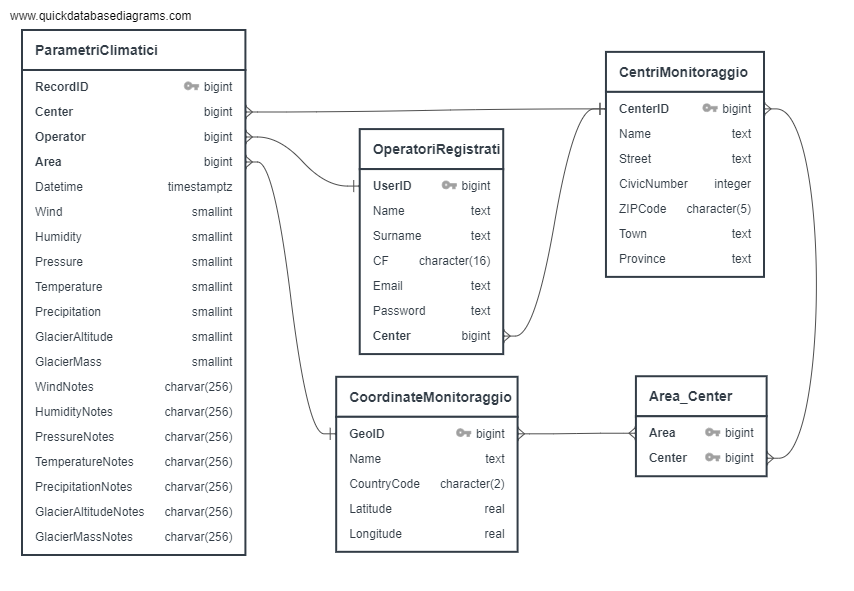
\includegraphics[width=0.9\linewidth]{../../../UniLab-server/QuickDBD-clima}
	\end{figure}
	
	Gli attributi di ogni relazione sono stati inseriti sulla base delle indicazioni fornite nel documento delle specifiche di progetto. Al riguardo, sono degne di nota le seguenti scelte progettuali:
	\begin{itemize}
		\item in \textit{\textbf{ParametriClimatici}}, è stato aggiunto l'attributo \textit{"RecordID"}, utilizzato come chiave primaria della relazione, in modo da usufruire di un identificatore univoco per ogni record che riguarda le misurazioni climatiche; inoltre gli attributi riguardanti le note dei parametri di rilevazione non sono stati dichiarati \textit{"NULLABLE"}, in quanto l'eventuale mancanza di tali dati (opzionali) è stata gestita a livello applicativo tramite l'uso di stringhe vuote;
		\item in \textit{\textbf{CoordinateMonitoraggio}}, gli attributi \textit{"Latitude"} e \textit{"Longitude"} sono stati separati, nonostante nel documento \textit{"CoordinateMonitoraggio.xlsx"} (fornito nelle specifiche di progetto, sulla base del quale è stata costruita questa relazione) siano parte dello stesso campo \textit{"Coordinates"}, in modo da facilitarne la manipolazione a livello applicativo.
	\end{itemize}
	
\chapter{Modulo serverCM}
\chapter{Modulo clientCM}
\nocite{IuriTex}
\bibliographystyle{alpha}
\bibliography{bib/biblio}
